
\documentclass{article}
\usepackage[utf8]{inputenc}
\usepackage{graphicx}  % For including images
\usepackage{geometry}  % For adjusting margins and spacings
\usepackage{enumitem}
\usepackage{float}
\usepackage{hyperref}

\usepackage{fancyhdr}
\pagestyle{fancy}
\fancyhf{} % Clear all headers and footers
\renewcommand{\headrulewidth}{0.4pt} % Add a rule below the header

\title{User Interface Design \& Evaluation}

\lhead{Name: Christopher Nowacki}
\chead{Class: CIS 280}
\rhead{User Interface Design \& Evaluation}
\geometry{top=2.5cm, bottom=2cm, left=2cm, right=2cm, headheight=15pt}

\begin{document}
\thispagestyle{fancy}

\section*{Part II}

\begin{enumerate}
    \item How would you define usability?

    \begin{quote}
    I would define usability in the context of UI design as a measurement of how easy users of a system can learn, understand and navigate a product and can successfully use a product to achieve whatever goal's they are using it for with minimal frustrations. From a UI perspective, a product should be intuitive, efficient, and hopefully somewhat pleasant to use.
    \end{quote}

    \item How would you measure a system's usability? Suppose your development team has created a prototype of a UI for a new system. Describe how you might test and measure the usability of your UI.

    \begin{enumerate}[label=\arabic*.]
        \item Find representative users -- preferable people whose experience aligns with the potential user base.
        \item Come up with a representative task. For an e-commerce site, it might be something like finding an item, adding it to the cart, and going through the checkout process.
        \item Record and observe how the user interacts with the system -- find spots where the UI is intuitive and the user has no problem -- also find spots where they have trouble with the interface.
    \end{enumerate}

    \item Describe the differences between UI design in a web environment and UI design in a desktop environment. Are there good / bad deeds in UI design that would be important for a desktop system but not for a browser-based system?

    \begin{quote}
    Desktop applications can full access to the resources on the machine/server they run on. This can mean improved performance. Web apps may be constrained by the limits of the browser they run in and may not have full access to resources. Given this, desktop applications may run "snappier" and be more responsive. Browser compatability and response design is important for browser-based systems. They need to be able to run a number of different browsers and need to have good design at multiple sizes/resolutions. Users can likely be more forgiving of small issues in a browser-based system. Users of a desktop application will expect a rich, responsive, and more powerful UI and will be less forgiving of poor performance.
    \end{quote}

    \newpage
    \item Usability-related IT jobs are now common. Add 3 usability jobs to your IT jobs table from Assignment 1. Examples: Usability Engineer, Usability Researcher, Human Factors Analyst.
    
      \begin{figure}[H]
        \centering
        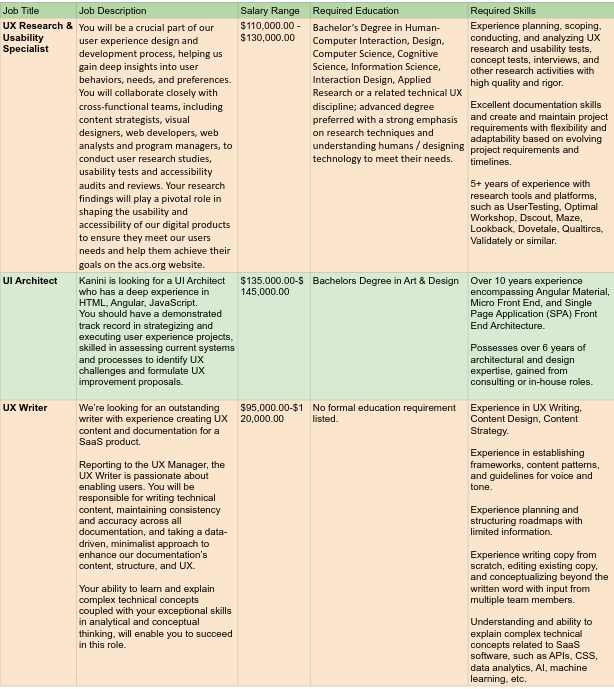
\includegraphics[width=0.8\linewidth]{images/job_listings.png}
        \caption{UI-Related Job Listings}
      \end{figure}
    \item What is a prototype? What can be learned from building a prototype of a proposed system?

    \begin{quote}
    A prototype is a model of a proposed product. Developing a prototype can help you answer important questions: Is my product feasible? What will my product look like for a user? How will my user interact with the system? These are things you should already have in mind -- but the prototype will help expose any holes or shortcomings you may have overlooked.
    \end{quote}

    \item What is User Testing? Look online for a description of a large company's User Testing lab.

    \begin{quote}
    The Usability Labs determine how useful products are by attempting to provide answers to three equally important questions: Does the product do something customers want? Can people use the product to do what it is designed to do? Is the product desirable?
    \end{quote}

    \item Describe the lab's layout \& the testing process.

    \begin{quote}
    To answer these questions, the Usability Labs employs engineers with a wide variety of educational backgrounds, including human-factors psychology, social psychology, industrial engineering, technical communications, developmental psychology, information science and computer science. A separate group, the Usability Test Coordinators, recruit outside users to spend a few hours at the Microsoft corporate campus working with the products Microsoft is developing. The Usability Engineers and Test Coordinators work closely together to bring in users whose work and experience are appropriate for the product they’ll be testing. By observing customers actually using a product, the engineers can determine how well the product meets their needs and whether it is easy to use.
    \end{quote}

    \item What is Heuristic Evaluation? What are its advantages \& disadvantages compared with User Testing?

    \begin{quote}
    Heuristic evaluation is a method for identifying design problems in a user interface. It differs with User Testing in that it is conducted by an usability expert. The design is judged against a set of guidelines (heuristics). It's advantages include: More cost-effective, Can be done more quickly, Early Identification: Issues can be caught early in design. Disadvantages include: May miss issues real users might encounter, Dependent on experts' expertise, Limited Feedback, may not give a good picture of usability and satisfaction for user.
    \end{quote}
\end{enumerate}

\end{document}

